%%% DOCUMENT SETUP %%%
\documentclass[11pt,a4paper]{article}
\usepackage[english]{babel}

%%% LAYOUT %%%
\usepackage{fullpage}
\usepackage[parfill]{parskip}
\usepackage{multicol}
\usepackage{footnote}

%%% GRAPHICS %%%
\usepackage{graphicx}
\usepackage{color}
\usepackage{graphics}
\usepackage{rotating}
\usepackage{subfig}
\usepackage{amsmath}
\usepackage{amssymb}
\usepackage{amscd}
\usepackage{xfrac}
\usepackage{float}
\usepackage{dsfont}

%%% FONT %%%
\usepackage{ifxetex}
\ifxetex
  \usepackage{fontspec}
    \setmainfont{Linux Libertine O}
  \usepackage{xunicode}
  \usepackage{microtype}
\else
  \usepackage[T1]{fontenc}
  \usepackage[latin1]{inputenc}
  \usepackage{times}
  \usepackage{microtype}
\fi

%%% Coding %%%
\usepackage{listings}
\usepackage{pseudocode}

%%% TITLE PAGE %%%
\author{Jeroen Hofman \ \ \ \ \ Carlo Kuiper\\
[15pt] University of Amsterdam (\textsc{UvA})}

\title{Computational Finance\\
  Assignment I: Black-Scholes Model and Binomial Tree Methods.}

\begin{document}
\maketitle
\captionsetup{width=0.8\textwidth}
\thispagestyle{empty}

%%% TABLE OF CONTENTS %%%
\newpage
\tableofcontents
\newpage

\section{Part 1: Option valuation}

In the first part of the assignment we look at the model for a binomial tree. We describe the theory behind it and the algorithm that is used. We also look at the derivation of the Black-Scholes model and compare the values given by this model with the binomial tree. We calculate option prices in the binomial tree model with different sets of parameters.

\subsection{Binomal Tree}
\subsubsection{Theory}
We use the binomial tree method to calculate the price of an option. This model implements the results of a multi-period binomial tree to simulate the stock price. How does it exactly work?

At each step, the stock price moves either up by a factor $u$ with a probability $p$ or moves down by a factor $d$ with a probability $1-p$. So if $S$ is the current price, then in the next period the price will either be $S_{up}=u S$ with probability $p$ or $S_{down}=dS$ with probability $1-p$. There is also a known risk free interest rate $r$ (with continuous compunding). To use this tree we need to specify the length of each period and the values of $u,d$ and $p$.

We divide the lifetime of an option $[0,T]$ in equal periods $\delta t$ and evaluate the option price after each of these time steps. To determine the values of the variables we use three equations:

First, we want to have an equality between the expected pay-off from a stock, $\mathbb{E}S$, and an equal risk neutral investment $S e^{r\delta t}$. Else there will be an arbitrage possibility. So $S e^{r\delta t}=puS+(1-p)dS$, or more conveniently $e^{r\delta t}=pu+(1-p)d$.

Second, we take the standard deviation equal to $\sigma$, the volatility of the stock. This means that the variance, $(\text{standard deviation})^2$, over a single period equals $\mathbb{E}S^2-(\mathbb{E}S)^2$. So $\sigma^2\delta t=pu^2+(1-p)d^2-(pu+(1-p)d)^2$.

Third, we want to have a recombining tree and choose $u=1/d$. Then the nodes will increase with $n+1$ instead of $2^n$.

We take our variables $u,d$ and $p$ such that these equations are satisfied. This was proposed by Cox, Ross and Rubinstein \cite{rubinstein}:

\begin{align}
u&=e^{\sigma\sqrt{\delta t}}\nonumber \\
d&=e^{-\sigma\sqrt{\delta t}}\nonumber \\
p&=\frac{a-d}{u-d} \quad \text{with } a=e^{r\delta t}
\end{align}

It is usefull to note that $1-p=\frac{u-a}{u-d}$. We will show that these variables satisfy the above formulated equations in the limit case of $\delta t$ going to zero. Starting with the first equation:

\begin{equation}
pu+(1-p)d=\frac{a-d}{u-d} u + \frac{u-a}{u-d} d = a = e^{r\delta t}
\end{equation}

For the second equation we need to use that $\delta t$ goes to zero. But first some algebra:

\begin{equation}
pu^2+(1-p)d^2-(pu+(1-p)d)^2 = (u-d)^2p(1-p)=(a-d)(u-a)
\end{equation}

The Talyor expansion of $a-d$ around zero is $1+r\delta t+\frac{r^2(\delta t)^2}{2}+\ldots-1+\sigma \sqrt{\delta t}-\frac{\sigma^2\delta t}{2}+\ldots$ and the Taylor expansion of $u-a$ around zero is $1+\sigma \sqrt{\delta t}+\frac{\sigma^2\delta t}{2}+\ldots-1-r\delta t-\frac{r^2(\delta t)^2}{2}-\ldots$ We find that

\begin{equation}
(a-d)(u-a)=(\sigma\sqrt{\delta t}+r\delta t+\ldots)(\sigma\sqrt{\delta t}-r\delta t+\ldots)=\sigma^2\delta t+\mathcal{O}((\delta t)^\frac{3}{2})
\end{equation}

and thus, when $\delta t$ is sufficiently small $\sigma^2\delta t+\mathcal{O}((\delta t)^\frac{3}{2})=\sigma^2\delta t+0$.

Lastly the third equation holds:

\begin{equation}
u=e^{\sigma\sqrt{\delta t}}=\frac{1}{e^{-\sigma\sqrt{\delta t}}}=\frac{1}{d}
\end{equation}

\subsubsection{Method}
We can implement this multi-period binomial tree to calculate the expected stock price at each node $(i,j)$ in the tree, given by $S_{0}u^id^{i-j}$ where $S_{0}$ is the stock price at the first level of the tree (so $t = 0$), $i$ is the level in which the node is, and $j$ is the position of the node in the level, where $j \leq i$. 

%$u$ and $d$ are the expected upward and downward stock price movements, given by:
%
%\begin{align}
%  \label{eq:ud}
%  &u = e^{\sigma \sqrt{(\delta t)}} \nonumber \\
%  &d = e^{-\sigma \sqrt{(\delta t)}}
%\end{align}
%
%where $\sigma$ is the volatility of the market. 

The value of the option $f$ at the expiration date $T$, corresponding to tree level $N = \sfrac{T}{\delta t}$, is dependent on the option type and given by:

\begin{itemize}
\item 
  $\text{max}(0,S_{N,j} - K)$ for a call option.
\item
  $\text{max}(0,K - S_{N,j})$ for a put option.
\end{itemize}

where $S_{N,j}$ is the stock price at node $j$ at level $N$ and $K$ is the strike price of the option. Given that we now have the option value at maturity of the contract, we can use risk-neutral valuation to calculate the option value at the previous time-step, where the option value at node $(i,j)$ is given by:

\begin{equation}
  \label{eq:f}
  f_{i,j} = e^{-r \delta t}(p f_{i+1,j+1} + (1 - p) f_{i+1,j})
\end{equation}

%where $r$ is the risk-free interest rate and $p$ is given by:
%
%\begin{equation}
%  \label{eq:p}
%  p = \frac{e^{r \delta t} - d}{u - d}
%\end{equation}
%
%where this can be derived from the risk-free approach. 

By using Equation \ref{eq:f} we can calculate the option value starting from the last level of the tree and work back to the first level to calculate $f_{1,1}$, which will be the option price at time zero.

Variables $u,d$ and $p$ completely determine the backward induction scheme. Equation \ref{eq:f} is then used to calculate the option price, however this is only valid for European options, which can only be exercised at maturity. If one considers American options, exercition is possible at any time between 0 and $T$ and hence Equation \ref{eq:f} is modified to:

\begin{align}
&f_{i,j} = \max(e^{-r \delta t}(p f_{i+1,j+1} + (1 - p) f_{i+1,j}),S_{N,j} - K) \; \text{for a call option, and} \nonumber \\
&f_{i,j} = \max(e^{-r \delta t}(p f_{i+1,j+1} + (1 - p) f_{i+1,j}),K - S_{N,j}) \; \text{for a put option} 
\end{align}

In principle the more steps we use in the tree, hence the smaller we make $\delta t$, the better the approximation for the option price. By changing the number of levels in the tree one can study the convergence of the option price.

If the values of the put and call options are calculated correctly, they should satisfy the put-call parity \cite{hull}, i.e.:

\begin{equation}
  c + K e^{-rT} = p + S_{0}
\end{equation}

where $c$ is the value of the European call option, and $p$ the value of the European put option. The put-call parity can be used to check the correctness of the results from the binomial tree backward induction scheme. In the case of American options there is an inequality ($\leq$), therefore it cannot be used to check the pricing of American options.

From the tree we obtain we can also calculate a hedge parameter $\Delta$, which is needed in the construction of a riskless portfolio, consisting of long $\Delta$ shares and short 1 option. $\Delta$ is calculated per branch of the tree and given by:

\begin{equation}
  \label{eq:deltadisc}
  \Delta_{i,j} = \frac{f_{i+1,j+1} - f_{i+1,j}}{S_{i+1,j+1} - S_{i+1,j}}
\end{equation}

Since $\Delta$ is different depending on the time step and the movement of the market, the holdings in the stock have to be adjusted periodically to maintain a riskless portfolio.

\subsection{Black Scholes model}
The binomial tree model equals the Black Scholes model in the limiting case when $\delta t$ goes to zero. In the Black Scholes model a stock price is simulated with the following formula:

\begin{equation}
\label{eq:bs}
\mathrm{d}S=rS\mathrm{d}t+\sigma S\mathrm{d}Z
\end{equation}

where $Z$ is a Wiener process. We recognize a Geometric Brownian mortion. By It\^o's formula we obtain the formula for the logarithm (It\^o's formula applied to the function $F(t,S)=\log S$)

\begin{equation}
\mathrm{d}\log S=\left(r-\frac{1}{2}\sigma^2\right)\mathrm{d}t+\sigma\mathrm{d}Z
\end{equation}

At the end of the time interval $[0,T]$, the Wiener process $Z$ is normally distributed with mean $0$ and variance $\sigma \sqrt{T}$, therefore $\log S_t$ is distributed as:

\begin{align}
\label{eq:dist}
\log S_t-\log S_0&\sim(r-\frac{1}{2}\sigma^2)T+\mathcal{N}(0,\sigma^2 T)\nonumber \\
\log S_t&\sim\mathcal{N}((r-\frac{1}{2}\sigma^2)T+\log S_0,\sigma^2 T)
\end{align}

We introduce the constants $\hat{\mu}=(r-\frac{1}{2}\sigma^2)T$ and $\hat{\sigma}=\sigma \sqrt{T}$. Then $\log S_t$ is normally distributed with mean $\hat{\mu}+\log S_0$ and variance $\hat{\sigma}$.

It was proven by Cox, Ross and Rubinstein in 1979 that the multi-period binomial tree converges to the Black Scholes model. Therefore the option prices of the binomial tree method converge to the prices found analytically using the Black Scholes model. The choice of parameters is not trivial, so the result is remarkable. The proof of convergence is quite long and can be found online (\cite{stat}). A different approach is to simulate the logarithm of the stock with a multi-period binomial tree. The equations become $pu+(1-p)d=\left(r-\frac{1}{2}\sigma^2\right)\delta t$, $pu^2+(1-p)d^2-\left(\left(r-\frac{1}{2}\sigma^2\right)\delta t\right)^2=\sigma^2\delta t$ and $u=\frac{1}{d}$. With the Central Limit Theorem it is clear that this converges to the logarithm of a stock used in the Black Scholes model (determining the variables is again not trivial).

With the Black Scholes model we can derive the value of a call option at time 0 analytically, we name it $c$. The value of a call option at time 0 is the discounted value of the stock price at time $T$, we also introduce the stochastic variabe $x_t=(\log S_t-\hat{\mu})/\hat{\sigma}$, or $S_t=e^{x_t\hat{\sigma}+\hat{\mu}}$ so that $x_t \sim \mathcal{N}(0,1)$ with standard normal distribution $\phi(x_t)$.

\begin{align}
c&=e^{-rT}\mathbb{E}\left[(S_T-K)^+\right]\nonumber \\
&=e^{-rT}\mathbb{E}\left[\left(e^{x_T\hat{\sigma}+\hat{\mu}}-K\right)^+\right]\nonumber \\
&=e^{-rT}\int_{\frac{\log K -\hat{\mu}}{\hat{\sigma}}}^{\infty}{e^{x_T\hat{\sigma}+\hat{\mu}}\phi(x_T)}\mathrm{d}x_T-e^{-rT}K\int_{\frac{\log K -\hat{\mu}}{\hat{\sigma}}}^{\infty}{\phi(x_T)}\mathrm{d}x_T
\end{align}

We take $x=x_T$, manipulating $e^{x_T\hat{\sigma}+\hat{\mu}}\phi(x)$ allows us to rewrite it as $e^{\hat{\mu}+\frac{\hat{\sigma^2}}{2}}\phi(x-\hat{\sigma})$.

\begin{equation}
e^{x_T\hat{\sigma}+\hat{\mu}}\phi(x)=\frac{1}{\sqrt{2\pi}}e^{-\frac{x^2-2x\hat{\sigma}-2\hat{\mu}}{2}}=\frac{1}{\sqrt{2\pi}}e^{-\frac{(x-\hat{\sigma})^2-2\hat{\mu}-\hat{\sigma}^2}{2}}=e^{\hat{\mu}+\frac{\hat{\sigma^2}}{2}}\phi(x-\hat{\sigma})
\end{equation}

Implementing this yields (we also use that $1-\mathcal{N}(x)=\mathcal{N}(-x)$),

\begin{align}
c&=e^{-rT}\int_{\frac{\log K -\hat{\mu}}{\hat{\sigma}}}^{\infty}{e^{\hat{\mu}+\frac{\hat{\sigma^2}}{2}}\phi(x-\hat{\sigma})}\mathrm{d}x-e^{-rT}K\int_{\frac{\log K -\hat{\mu}}{\hat{\sigma}}}^{\infty}{\phi(x)}\mathrm{d}x \nonumber \\
&= e^{-rT+\hat{\mu}+\frac{\hat{\sigma^2}}{2}}\left(1-\mathcal{N}\left(\frac{\log K -\hat{\mu}}{\hat{\sigma}}-\hat{\sigma}\right)\right)-e^{-rT}K\left(1-\mathcal{N}\left(\frac{\log K -\hat{\mu}}{\hat{\sigma}}\right)\right)\nonumber \\
&= e^{-rT+\left(r-\frac{1}{2}\sigma^2\right)T+\frac{1}{2}\sigma^2T+\log S_0}\left(\mathcal{N}\left(\frac{-\log K +\hat{\mu}}{\hat{\sigma}}+\hat{\sigma}\right)\right)-e^{-rT}K\left(\mathcal{N}\left(\frac{-\log K +\hat{\mu}}{\hat{\sigma}}\right)\right)
\end{align}

Next we fill in the values of $\hat{\mu}$ and $\hat{\sigma}$.

\begin{align}
\label{eq:callprice}
c&= S_0 \mathcal{N}\left(\frac{\log\left(\frac{S_0}{K}\right)+\left(r-\frac{1}{2}\sigma^2\right)T}{\sigma\sqrt{T}}+\sigma\sqrt{T}\right)-e^{-rT}K\mathcal{N}\left(\frac{\log\left(\frac{S_0}{K}\right)+\left(r-\frac{1}{2}\sigma^2\right)T}{\sigma\sqrt{T}}\right)\nonumber \\
&=S_0\mathcal{N}(d_1)-Ke^{-rT}\mathcal{N}(d_2)
\end{align}

with $d_1=\frac{\log\left(\frac{S_0}{K}\right)+\hat{\mu}}{\hat{\sigma}}$ and $d_2=d_1-\sigma \sqrt{T}$.

The $\Delta$ of a call option at time 0 can also be derived from the Black Scholes model. We will make use of the partial derivatives of $d_1$ and $d_2$ to the stock price at time 0.

$\frac{\partial d_1}{\partial S}=\frac{1}{\frac{{S}{K}}{\hat{\sigma}}}\frac{1}{K}=\frac{1}{S_0\hat{\sigma}}$ likewise $\frac{\partial d_1}{\partial S_0}=\frac{1}{S_0\hat{\sigma}}$

The $\Delta$ of a call is the partial derivative of a call option price to the stock price

\begin{align}
\Delta_0=\frac{\partial C}{\partial S}(0)&=\mathcal{N}(d_1)+S_0\phi(d_1)\frac{\partial d_1}{\partial S_0}-Ke^{-rT}\phi(d_2)\frac{\partial d_2}{\partial S_0}\nonumber \\
&=\mathcal{N}(d_1)+\frac{1}{\hat{\sigma}}\left(\phi(d_1)-\frac{K}{S_0}e^{-rT}\phi(d_1-\sigma\sqrt{T})\right)
\end{align}

We can manipulate the standard normal distribution $\phi(x)$ to get the equality, $\phi(d_1-\sigma \sqrt{T})=\phi(d_1)e^{d_1\sigma\sqrt{T}-\frac{\sigma^2T}{2}}$.

\begin{equation}
\phi(d_1-\sigma \sqrt{T})=\frac{1}{\sqrt{2\pi}}e^{-\frac{(d_1-\sigma\sqrt{T})^2}{2}}=\frac{1}{\sqrt{2\pi}}e^{-\frac{d_1^2}{2}+d_1\sigma\sqrt{T}-\frac{\sigma^2T}{2}}=\phi(d_1)e^{d_1\sigma\sqrt{T}-\frac{\sigma^2T}{2}}
\end{equation}

Implementing this yields us the desired result.

\begin{align}
\label{eq:delta}
\Delta_0&=\mathcal{N}(d_1)+\frac{\phi(d_1)}{\hat{\sigma}}\left(1-\frac{K}{S_0}e^{-rT+d_1\sigma\sqrt{T}-\frac{\sigma^2T}{2}}\right)\nonumber \\
&=\mathcal{N}(d_1)+\frac{\phi(d_1)}{\hat{\sigma}}\left(1-\frac{K}{S_0}e^{-rT+\log\left(\frac{S_0}{K}\right)+(r+\frac{1}{2}\sigma^2)T-\frac{\sigma^2T}{2}}\right)\nonumber \\
&=\mathcal{N}(d_1)+\frac{\phi(d_1)}{\hat{\sigma}}(0)\nonumber \\
&=\mathcal{N}(d_1)
\end{align}

\subsection{Measurements and Results}

As an example we consider an option in a stock with a maturity of one year and a strike price of 99. The one year interest rate is 6\% and the current stock price is 100. The volatility of the market is assumed to be 20\%.

Given the values above and the equations from the previous section, we can now construct a binomial tree consisting of $N$ layers, giving $\delta t = \sfrac{1}{N}$ since $T = 1$. We first look at a European call and put option with $N = 50$ and consider different values of the volatility $\sigma$. The results are given in the table below:

\begin{table}[H]
  \centering
  \begin{tabular}{l | l | l}
    $\sigma$ (\%) &Eur. call option price & Eur. put option price\\
    \hline
    5 & 6.9378 & 0.1725\\
    10 & 8.1387 & 1.3734\\
    15 & 9.7879 & 3.0226\\
    20 & 11.5697 & 4.8043\\
    25 & 13.4040 & 6.6387\\
    50 & 22.7270 & 15.9617\\
  \end{tabular}
  \caption{European call and put option prices for different values of $\sigma$ for a binomial tree with $N = 50$.}
  \label{tab:eucall}
\end{table}

Clearly if the volatility increases, the option prices are increasing as well. This is expected because in the case of a call, if the volatility is high, there is a lot of profit potentially to be made if the price of the stock goes up, however, if the price of the stock goes down, one simply does not exercise the option and hence only the option price is taken as a loss. So potentially there is a lot of money to be made in a market which goes up, but the losses are only the option price, regardless of how much the market goes down. The same reasoning holds for the put option, but here it is the other way around.

We can study the convergence of this option types as a function of the number of layers in the tree, $N$ and compare it with the Black-Scholes analytical value. Since the difference in the implementation of European/American call and put options is small, we can do this for all four option types. Figure \ref{fig:conv} shows the the option price as a function of $N$ and the Black-Scholes analytical value for European call and put options. 

\begin{figure}[H]
  \centering
  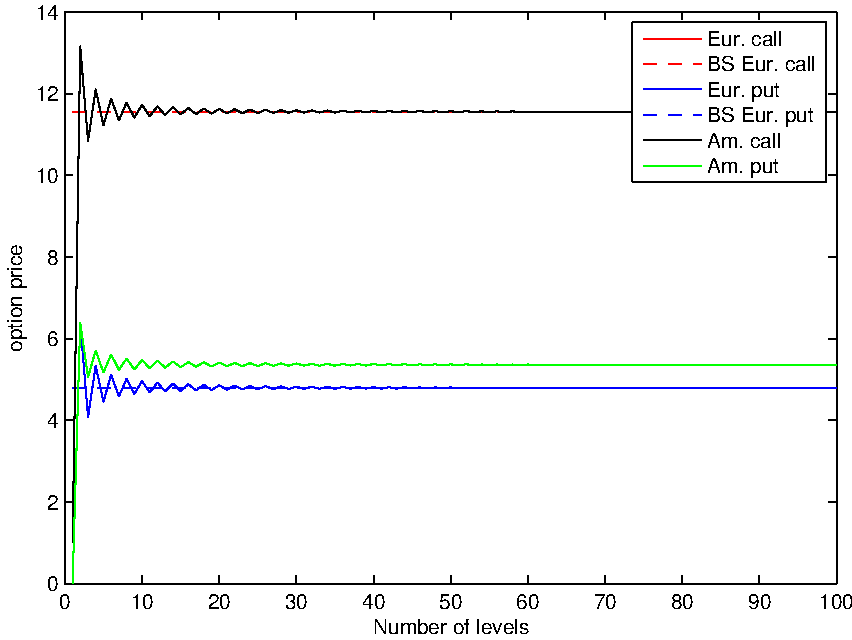
\includegraphics[width=0.7\textwidth]{conv.pdf}
  \caption{Option price (binomial tree and analytical) as a function of $N$.}
  \label{fig:conv}
\end{figure}

From the figure we see that the European call option and the American call option are behaving exactly the same. This is expected, since exercising the American call option before it reaches maturity is not wise, for two reasons:

\begin{itemize}
\item 
  A call option provides an insurance against the stock price falling below the exercise price, since in that case the call option is simply not exercised, while in the case of having the actual stock the investor looses money.
\item
  By not exercising before maturity the money to be paid can still be earned interest on.
\end{itemize}

For this reason the American call behaves like an European call and hence they are priced the same. Furthermore the American and European put options are priced lower than their call counterparts, this is because of the specific example we are looking at, which gives for European options (provided the put-call parity is satisfied, see below):

\begin{equation}
  c - p = S_{0} - K e^{-rT} = 100 - 99 e^{-0.06} > 0
\end{equation}

and for American call option price $C$ and put option price $P$:

\begin{equation}
  S_{0} - K \leq C - P \leq S_{0} - K e^{-rT}
\end{equation}

which gives $1 \leq C - P \leq 6.7653$ and hence $C > P$.

Furthermore the call-put parity is indeed satisfied in this example for European options, since we have ($N = 100$):

\begin{equation}
  c - p - S_{0} + K e^{-rT} = 11.5697 - 4.8043 - 100 + 99 e^{-0.06} = 4.8317 \;  10^{-13} \approx 0
\end{equation}

The value is not exactly zero, however this value converges to zero if $N$ is increased, since we obtain better approximations of the call and put price.

We also see that the American put option is worth more than the European put option, which is because the American version can be exercised earlier whereas it also has all the possibilities of the European put option, so hence its value will be higher.

From the figure we can see that the Black-Scholes analytical value is close to the binomial tree approximation. We can see the convergence of the binomial tree approximation to the analytical Black-Scholes value using the following table:

\begin{table}[H]
  \centering
  \begin{tabular}{l || c | c | c | c | c | c}
    N & B.S. Call & Binomial Call & Difference (\%) & B.S. Put & Binomial Put & Difference (\%)\\
    \hline
    50 & 11.5443 & 11.5697 & 0.2200 & 4.7790 & 4.8043 & 0.5294 \\
    100 & 11.5443 & 11.5522 & 0.0680 & 4.7790 & 4.7869 & 0.1653 \\
    1000 & 11.5443 & 11.5453 & 0.0087 & 4.7790 & 4.7800 & 0.0209 \\
    5000 & 11.5443 & 11.5445 & 0.0017 & 4.7790 & 4.7793 & 0.0042 \\ 
  \end{tabular}
  \caption{Analytical and binomial tree values and their relative difference (\%)}
  \label{tab:diff}
\end{table}

From the above table we see that the binomial tree approximation indeed converges to the Black-Scholes value if $N$ increases. This is also a verification that our binomial tree model is correct.

If we zoom in on the binomial tree for the European call option and show the results up to 1000 levels, see figure \ref{fig:closeup}, we see some extra oscillations next to the oscillation between odd and even levels of the tree (caused by the asymetry in the payoff). One can derive analytically that these oscillations do occur and that they consists of bounded functions which do not converge in the limit of large $N$. However the behavior of the binomial tree as a whole is a convergence in the order of $1/N$. For details we refer to \cite{diener}, since this is not the purpose of the assignment.

\begin{figure}[H]
  \centering
  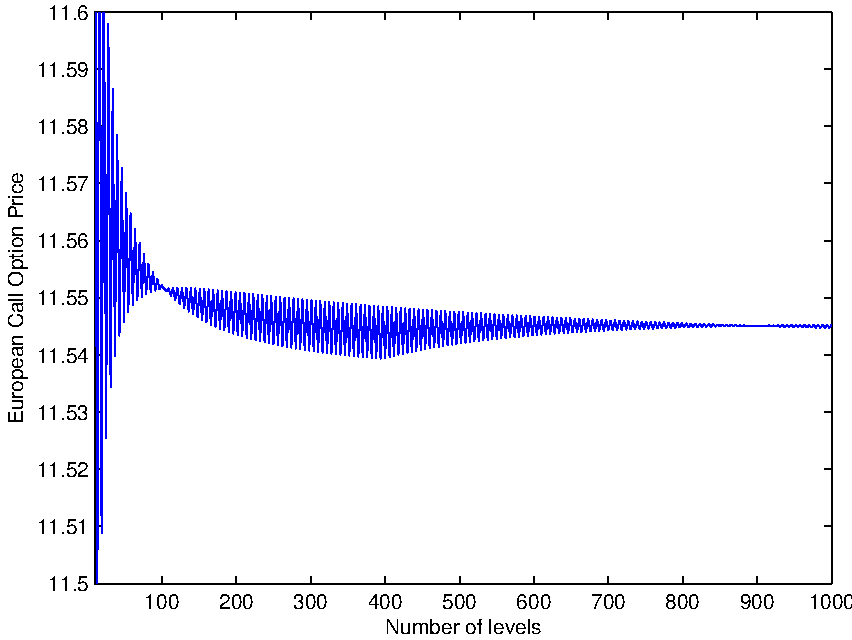
\includegraphics[width=0.7\textwidth]{closeup.pdf}
  \caption{Close up of the behavior of the European call option up to $N = 1000$.}
  \label{fig:closeup}
\end{figure}

Returning to the algorithm, the complexity can be divided into several parts:

\begin{itemize}
\item 
  Calculating the stock price: $C_{0} N(N+1)$, the size of the tree times a factor.
\item
  Calculating the option value at the final level: $C_{1} N$, the size of the last level.
\item
  Calculating the option value at all other nodes: $C_{2} (N-1)N$, the size of the tree minus the last level.
\end{itemize}

Combining these results and not caring about factors, we see that the complexity of our problem is $\mathcal{O}(N^2)$, which makes sense since the tree can be seen as an lower triangle matrix of size NxN.

From the binomial tree we can calculate a hedge parameter $\Delta$, given by equation \ref{eq:deltadisc}. We are interested in the value of $\Delta$ at $t = \delta t$, i.e. the first timestep we are able to evaluate $\Delta$. We can calculate this value for different number of levels in the tree, the first value of $\Delta$ should converge to a certain value if the number of levels in the tree increases. Figure \ref{fig:delta} shown below gives the calculation of the value of $\Delta$ at the second level of the tree for increasing tree level.

\begin{figure}[H]
  \centering
  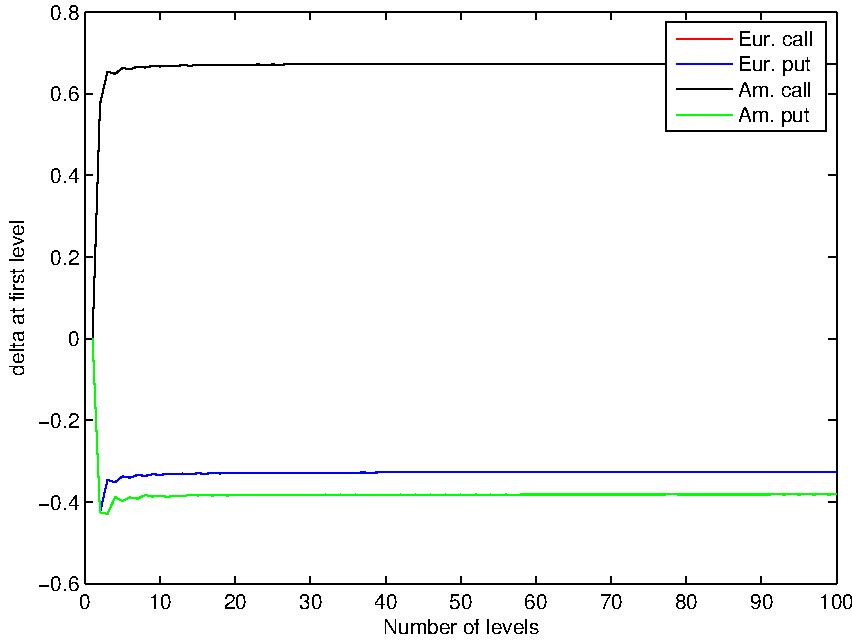
\includegraphics[width=0.7\textwidth]{delta.pdf}
  \caption{$\Delta$ at the second tree level as a function of total number of levels in the tree.}
  \label{fig:delta}
\end{figure}

From the figure we see indeed that $\Delta$ is converging for an increasing number of tree levels. The $\Delta$ value for American/European call option is positive (0.6732 for $N = 100$), while the value for an European put (-0.3268 for $N = 100$) and an American put (-0.3814 for $N = 100$) are negative. This is logical because of the $\Delta f$ in the definition, which will always be positive for calls and negative for puts, since the former has an increased option price by markets going up, and the latter by markets going down.

Lastly we look a little more closer at American options, we compute the option prices for a call and put option for the same volatilities and parameters as we reported for the European call option, we obtain the following results:

\begin{table}[H]
  \centering
  \begin{tabular}{l | l | l}
    $\sigma$ (\%) & Am. call option price & Am. put option price \\
    \hline
    5 & 6.9378 & 0.4109\\
    10 & 8.1387 & 1.8494\\
    15 & 9.7879 & 3.5637\\
    20 & 11.5697 & 5.3707\\
    25 & 13.4040 & 7.2202\\
    50 & 22.7270 & 16.5959\\
  \end{tabular}
  \caption{American call and American put option prices for different values of $\sigma$ for a binomial tree with $N = 50$.}
  \label{tab:amcall}
\end{table}

As we can see from the table, as the volatility increases the option prices increases, for the same reasons as mentioned earlier in the European case. Note that the European put price is always lower than the American put price, regardless of the value of the volatility.

\section{Part 2: Hedging Simulations}

In this section we will hedge an one-year European call option using $\Delta$ hedging. We will check the validity of the model as well as measure performance of the hedging with different time intervals.

\subsection{Method}

At time $T = 0$ we start with a stock price $S_0$, a given volatility of the market $\sigma$ and a strike price for a call $K$. We calculate the price of a call $c$ and the value $\Delta_0$ using the Black Scholes model, see equations \ref{eq:callprice} and \ref{eq:delta} above. We sell 1 call for the call price and we buy $\Delta$ shares for the current stock price to create a riskless portfolio. The amount of money that will be borrowed is $\text{debt}_0 = \Delta_0 \times S_0 - c$.  

Then we take steps in time, given by $\delta t$, and calculate the new stock price at each timestep, given by the discretization of equation \ref{eq:bs}, using the random variable $dZ \sim \mathcal{N}(0,\sqrt{\delta t})$. With the new stock price we calculate the new call price and a new $\Delta$ using again Black-Scholes. We sell the $\Delta$ shares from the previous time step for the current stock price and buy the new $\Delta$ shares for the current stock price. The new value of the loan will be:

\begin{equation}
  \label{eq:loan}
  \text{debt}_{i} = \text{debt}_{i-1} e^{r\delta t} + (\Delta_{i} - \Delta_{i-1}) S_i
\end{equation}

where $r$ is the risk-free interest rate. We repeat this procedure, keeping $\delta t$ fixed, until the contract reaches maturity. At the last time step when $t = T$ we do not invest anymore in new shares so the $\Delta_i$ term in the above equation is zero. Furthermore we have to pay the buyer of the call the difference between the strike price $K$ and the current stock price $S_T$, given by $\text{max}(S_T - K,0)$ (the payoff for a call). If the hedging is done correctly and $\delta t$ is sufficiently small, the hedging party should have no net loss or gain at the end of the procedure. 

In this algorithm there are two volatilities present: the volatility in the movement of the stock price given by equation \ref{eq:bs}, hereafter referred to as $\sigma_S$ and the volatility used in the Black-Scholes model given by equations \ref{eq:callprice} and \ref{eq:delta}, hereafter referred to as $\sigma_{BS}$. We can look at different values of these volatilities, namely we can distinguish three different domains:

\begin{itemize}
\item 
  $\sigma_S = \sigma_{BS}$: both volatilities are the same, this should give the best result for the hedging procedure.
\item
  $\sigma_S > \sigma_{BS}$: the volatility in the stock price is higher than the volatility in the model, so the model underestimates.
\item
  $\sigma_S < \sigma_{BS}$: the volatility in the stock price is lower than the volatility in the model, so the model overestimates.
\end{itemize}

\subsection{Measurements and Results}

We performed measurements on the delta hedging simulation with the following parameters:

\begin{itemize}
\item 
  $S_0 = 100$
\item
  $K = 99$
\item
  $r = 0.06$
\item
  $\sigma_S = \sigma_{BS} = 0.20$ (case I), $\sigma_S = 0.19, \sigma_{BS} = 0.20$ (case II) and $\sigma_S = 0.21, \sigma_{BS} = 0.20$ (case III)
\item
  $\delta t = 1/52$ (weekly), $\delta t = 1/104$ (biweekly) $\delta t = 1/365$ (daily, naively assuming 365 business days)
\end{itemize}

For a single simulation we can measure the stock price $S$, the call price $c$, the $\Delta$ and the loan. Such a measurement is done in the figure \ref{fig:hedge} below, using the case of $\sigma_S = \sigma_{BS}$ and using daily hedging. We see that all four graphs make more or less the same movement, i.e. more or less a continuous slope up. The value for $\Delta$ goes to 1 as the time to maturity decreases, because $\Delta S \approx \Delta c$ for $t \rightarrow T$. If the time to maturity is large, a change in stock price will not give an exact same change in call price, since the stock price at maturity might still be very different. However, when we approach maturity, an increase or decrease in the stock price leads to an equal increase or decrease in the call price since it is highly likely the stock price will end up in such a state due to the short time to maturity. If the option is out of the money shortly before maturity (so the stock price is lower than the strike price), $\Delta$ will go to zero because a change in stock price does not lead to a change in the call price, since the option will be worthless.

\begin{figure}[H]
  \centering
  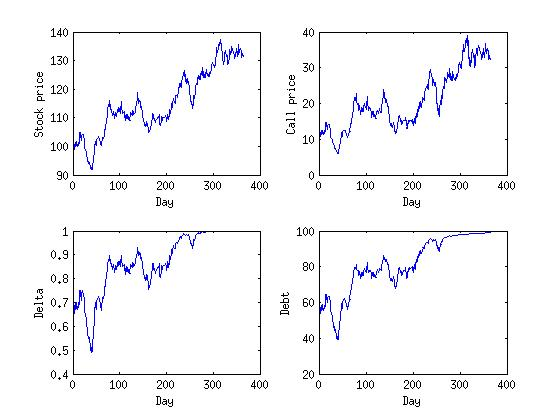
\includegraphics[width=0.7\textwidth]{hedge.jpg}
  \caption{Example of a daily hedging simulation.}
  \label{fig:hedge}
\end{figure}

This is just an example of one simulation, we want many simulations to calculate the mean debt at the end as well as the error on this debt. Therefore we measured the mean debt and the error on the mean debt (with a 95\% confidence interval) over 1000 simulations, going through all the options given above. The results are given in Table \ref{tab:hedge} below:

\begin{table}[H]
  \centering
  \begin{tabular}{l | c | c | c}
    \hline
    $\delta t$ & $\sigma_S = \sigma_{BS}$ & $\sigma_S < \sigma_{BS}$ & $\sigma_S > \sigma_{BS}$ \\
    \hline
    1/52 & $-0.0391 \pm 0.0568$ & $-0.3972 \pm 0.0553$ & $0.4224 \pm 0.0645$\\
    1/104 & $-0.0342 \pm 0.0413$ & $-0.4092 \pm 0.0415$ & $0.3605 \pm 0.0427$\\
    1/365 & $0.0011 \pm 0.0215$ & $-0.3677 \pm 0.0225$ & $0.4017 \pm 0.0249$\\
    $\delta t \rightarrow 0$ & $0$ & $-0.3594$ & $0.3614$\\
  \end{tabular}
  \caption{Results for the hedging and the standard error for different values of the volatilities and different $\delta t$.}
  \label{tab:hedge}
\end{table}

From the table we see that as the hedging frequency increases, the error becomes smaller. This shows that is indeed wise to have a high hedging frequency, since this makes the portfolio more riskless. The total expected debt at time $T$ converges to certain values. They can be found in the bottom line of the table. The values come from a formula which can be derived in the following way:

\begin{align}
\text{Expected debt at $T$}=~&\mathbb{E}[\text{initial hedging costs}]+\sum_{i=1}^{N-1}\mathbb{E}[\text{hedging costs at $i\delta t$}]+\mathbb{E}[\text{final hedging costs}] \nonumber \\
=&~\mathbb{E}[\Delta_0S_0-c]+\sum_{i=1}^{N-1}\mathbb{E}[(\Delta_i-\Delta_{i-1})S_i|\mathcal{F}_{i\delta t}]+\mathbb{E}[c(T)-\Delta_{N-1}S_T|\mathcal{F}_{T}]
\end{align}

The expectation of the stock price will be assumed to follow the formula $\mathrm{d}S=rS\mathrm{d}t+\sigma_{BS}S\mathrm{d}Z$. However in the filtration $\mathcal{F}_t$, `the history' up to time $t$, the stock price has followed the formula $\mathrm{d}S=rS\mathrm{d}t+\sigma_{S}S\mathrm{d}Z$. This means that $\mathbb{E}[(\Delta_i-\Delta_{i-1})S_i|\mathcal{F}_{i\delta t}]=\mathbb{E}[(\Delta_i-\Delta_{i-1})S_0e^{ri\delta t}|\mathcal{F}_{i\delta t}]$, $\mathbb{E}[c|\mathcal{F}_{T}]=c_S$ and that all $\Delta$'s are constants. Consequently:

\begin{align}
\text{Expected debt at $T$}=&~\Delta_0S_0e^{rT}-c_{BS}+\sum_{i=1}^{N-1}(\Delta_i-\Delta_{i-1})S_0e^{ri\delta t}e^{r(T-i\delta t)}+c_S-\Delta_{N-1}S_0e^{rT} \nonumber\\
=&~c_S-c_{BS}
\end{align}

with $c_S$ the call price when the stock has a volatility of $\sigma_S$ en $c_{BS}$ when the stock has a volatility of $\sigma_{BS}$. The result makes sense. With the portfolio a call option is replicated under the Black-Scholes parameters, however the option behaves under the stock price parameters, therefore you will pay for a $c_{BS}$ and get a $c_S$. We see in the table that the values converge to the value given by the equation above as $\delta t$ becomes smaller, except when $\sigma_S > \sigma_{BS}$, for which we were not able to find an explanation.

We can furthermore verify that our algorithm for the stock price is correct by making a histogram of the distribution of the log of the stock prices at maturity of the call contract. According to the Black-Scholes model the log of the stock price has a distribution equal to $\mathcal{N}((r-\sfrac{1}{2}\sigma^2)T + \text{log}S_0,\sigma^2T)$, see equation \ref{eq:dist}. In figure \ref{fig:dist} below a histogram is plotted for the log of the stock prices at maturity of the call contract, together with the theoretical distribution according to the Black-Scholes model. The parameters which are used are the same as stated in the list above, we used $\delta t = 1/365$ and $\sigma_S = \sigma_{BS}$. We measured the stock price at maturity $10^4$ times. The figure shows that indeed the sampling for the stock price used in the delta hedging follows a lognormal distribution, since the theoretical curve and the histogram show the same distribution.

\begin{figure}[H]
  \centering
  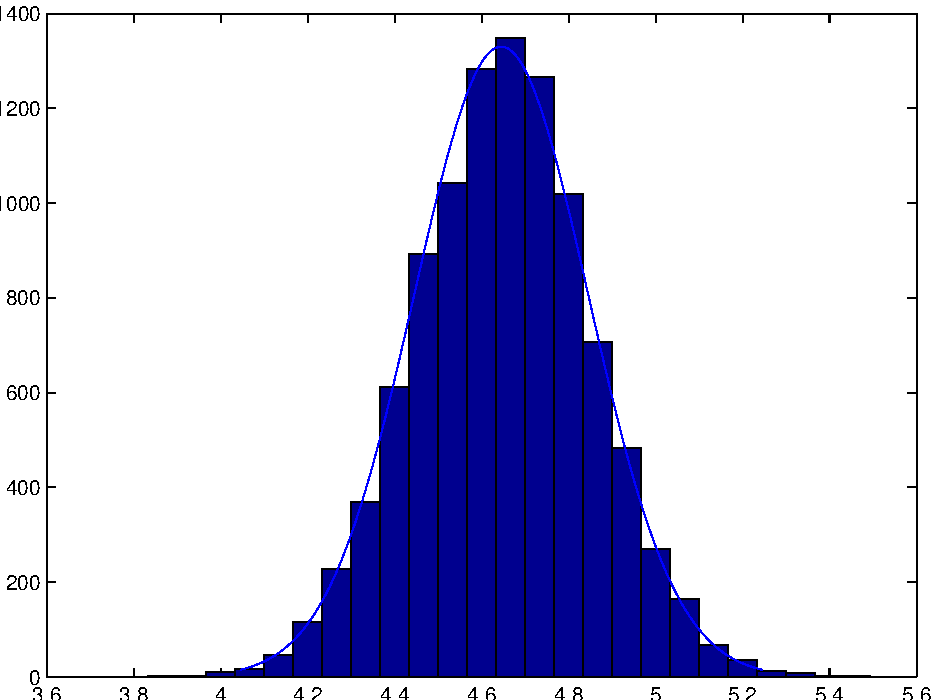
\includegraphics[width=0.7\textwidth]{dist.pdf}
  \caption{Distribution of the log of the stock prices at maturity together with the theoretical prediction using Black-Scholes (solid line).}
  \label{fig:dist}
\end{figure}

In practice $\sigma_{BS}$ is often chosen based upon historical values and then updated as new values of the stock price become available. Given the historical values $S_{-T},S_{\delta t-T},\ldots,S_0$ we can compute the desired volatility by taking the square root of the (unbiased) sample variance estimate,

\begin{equation}
\sigma_{BS}^2=\frac{\sum_{i=1}^N S_{i\delta t-T}-S_{(i-1)\delta t-T}-\left(\sum_{i=1}^N S_{i\delta t-T}-S_{(i-1)\delta t-T}\right)^2}{n-1}
\end{equation}

When a new stock price becomes available. There are two cases. When the stock price is expected to be constant, the more measurements the better. The historic volatility will be calculated with

\begin{equation}
\sigma_{BS}^2=\frac{\sum_{i=1}^{N+1} S_{i\delta t-T}-S_{(i-1)\delta t-T}-\left(\sum_{i=1}^{N+1} S_{i\delta t-T}-S_{(i-1)\delta t-T}\right)^2}{n}
\end{equation}

However, when the stock price is not expected to be constant, the older measurements become outdated. A volatility that can be used comes from

\begin{equation}
\sigma_{BS}^2=\frac{\sum_{i=2}^{N+1} S_{i\delta t-T}-S_{(i-1)\delta t-T}-\left(\sum_{i=2}^{N+1} S_{i\delta t-T}-S_{(i-1)\delta t-T}\right)^2}{n-1}
\end{equation}

When more stock price measurents become available both methods can be updated accordingly. These are just a few of the methods to calculate the historic volatility.

\section{Conclusion}

We discussed the theory behind the Black-Scholes model and a discrete approximation: the binomial tree method for option pricing. We found that the price calculated with the binomial tree method converges to the Black-Scholes price. Our model was verified by checking the put-call parity (and its counterpart for American style options). Furthermore we noticed an increase in the option price when the volatility of the underlying is increased. We also implemented a second model, delta hedging. There, an option is replicated with stocks at fixed time steps according to the Black-Scholes dynamics to create a riskless portfolio. We found that increasing the hedging frequency yields results closer to 0, meaning a more precise hedge. If the stock volatility is not equal to the volatility used in Black-Scholes the results will become closer to a difference between two specific call options.

\begin{thebibliography}{10}
\bibitem{rubinstein} 
  J.C. Cox, et al., \emph{Option Pricing: A Simplified Approach}, 1979, Journal of Financial Economics, Vol. 7, 229-263

\bibitem{hull}
  J.C. Hull, \emph{Options, Futures and Other Derivatives (6th ed.)}, 2005, Prentice-Hall, ISBN 0131499084

\bibitem{diener}
  F. Diener, M. Diener, \emph{Asymptotics of the price oscillations of a European call option in a tree model}, 2004, Mathematical Finance, Vol. 14. No. 2, 271-293

\bibitem{stat}
  http://www.stat.unc.edu/faculty/cji/890-11/L4.pdf

\end{thebibliography}

\end{document}
